% mnras_template.tex 
%
% LaTeX template for creating an MNRAS paper
%
% v3.0 released 14 May 2015
% (version numbers match those of mnras.cls)
%
% Copyright (C) Royal Astronomical Society 2015
% Authors:
% Keith T. Smith (Royal Astronomical Society)

% Change log
%
% v3.0 May 2015
%    Renamed to match the new package name
%    Version number matches mnras.cls
%    A few minor tweaks to wording
% v1.0 September 2013
%    Beta testing only - never publicly released
%    First version: a simple (ish) template for creating an MNRAS paper

%%%%%%%%%%%%%%%%%%%%%%%%%%%%%%%%%%%%%%%%%%%%%%%%%%
% Basic setup. Most papers should leave these options alone.
\documentclass[fleqn, usenatbib]{mnras}

% MNRAS is set in Times font. If you don't have this installed (most LaTeX
% installations will be fine) or prefer the old Computer Modern fonts, comment
% out the following line
%\usepackage{newtxtext,newtxmath}
% Depending on your LaTeX fonts installation, you might get better results with one of these:
\usepackage{mathptmx}
%\usepackage{txfonts}

% Use vector fonts, so it zooms properly in on-screen viewing software
% Don't change these lines unless you know what you are doing
\usepackage[T1]{fontenc}

% Allow "Thomas van Noord" and "Simon de Laguarde" and alike to be sorted by "N" and "L" etc. in the bibliography.
% Write the name in the bibliography as "\VAN{Noord}{Van}{van} Noord, Thomas"
%\RobustCommand{\VAN}[3]{#2}
%\let\VANthebibliography\thebibliography
%\def\thebibliography{\DeclareRobustCommand{\VAN}[3]{##3}\VANthebibliography}


%%%%% AUTHORS - PLACE YOUR OWN PACKAGES HERE %%%%%

% Only include extra packages if you really need them. Common packages are:
\usepackage{graphicx}	% Including figure files
\usepackage{amsmath}	% Advanced maths commands
\usepackage{amssymb}	% Extra maths symbols
\usepackage[alsoload=astro]{siunitx}
%\usepackage[colorlinks,
%			bookmarks=true,
%			linkcolor=blue,
%			urlcolor=blue,
%			citecolor=blue
%			]{hyperref}
\usepackage{physics}
\usepackage{url}
%\usepackage[backend=biber,
%			style=authoryear,
%			natbib=true,
%			url=false, 
%			doi=true,
%			eprint=false,
%			useprefix=false,
%			maxbibnames=9,
%			maxcitenames=1,
%			uniquelist=minyear,
%			sorting=ynt
%			]{biblatex}
\usepackage{color}
\usepackage{multirow}
%%%%%%%%%%%%%%%%%%%%%%%%%%%%%%%%%%%%%%%%%%%%%%%%%%

%%%%% AUTHORS - PLACE YOUR OWN COMMANDS HERE %%%%%

% Please keep new commands to a minimum, and use \newcommand not \def to avoid
% overwriting existing commands. Example:
%\newcommand{\pcm}{\,cm$^{-2}$}	% per cm-squared
%\addbibresource{refs.bib}
\DeclareSIUnit\year{yr}
\DeclareSIUnit\h{\mathnormal{h}}
\newcommand{\hlight}[1]{(\color{red}#1\color{black}) }
\sisetup{separate-uncertainty = true,
	bracket-numbers=true}
\DeclareMathOperator{\sgn}{\operatorname{sgn}}
%%%%%%%%%%%%%%%%%%%%%%%%%%%%%%%%%%%%%%%%%%%%%%%%%%

%%%%%%%%%%%%%%%%%%% TITLE PAGE %%%%%%%%%%%%%%%%%%%

% Title of the paper, and the short title which is used in the headers.
% Keep the title short and informative.
\title[Effects of systematics on void BAO]{Analysis of the response of void BAO to systematic effects in the SDSS observations using mock datasets}

% The list of authors, and the short list which is used in the headers.
% If you need two or more lines of authors, add an extra line using \newauthor
\author[D. Forero-S\'anchez et al.]{
Daniel Forero-S\'anchez,$^{1}$\thanks{E-mail: daniel.forerosanchez@epfl.ch (DFS)}
\\
% List of institutions
$^{1}$\'Ecole Polytechnique F\'ed\'erale de Lausanne, Lausanne, Switzerland.\\
}

% These dates will be filled out by the publisher
\date{Accepted XXX. Received YYY; in original form ZZZ}

% Enter the current year, for the copyright statements etc.
\pubyear{2020}

% Don't change these lines
\begin{document}
\label{firstpage}
\pagerange{\pageref{firstpage}--\pageref{lastpage}}
\maketitle

% Abstract of the paper
\begin{abstract}
Baryon Acoustic Oscillations (BAO) were produced due to (baryonic) matter -- photon plasma oscillations in the early Universe and they are therefore encoded in its spatial 3-dimensional distribution. The signal imprinted recognizable in configuration space as a peak in the 2-point correlation function and in Fourier space as wiggles in the power spectrum. The BAO feature provides a standard scale that can be measured at different redshifts. In recent years, large volume galaxy surveys have dedicated efforts to the mapping of the large-scale structure by using different kinds of matter tracers (such as galaxies), however, these observations are always clouded by systematical effects coming from observational difficulties and instrument limitations. In the present work, we aim to evaluate the impact of these systematical effects in the void BAO signal in configuration space (as obtained from the discrete distribution of Emission Line Galaxies (ELG) using a Delaunay Triangulation algorithm) as opposed to the galaxy BAO. To do this we compute the optimal radius cut to separate voids-in-voids (bigger, true voids) from voids-in-clouds (smaller, dark matter-rich regions) and find it to be $R_c = \SI{15.5}{\h^{-1}\mega\parsec}$. We measure the BAO scale by fitting the dilation parameter to different models. Measurements hint towards a difference in the impact of systematics on voids vs. galaxies. Nonetheless the error is still relatively high to draw definitive conclusions. We measure, in the mean case, $\alpha_{\mathrm{all}} - \alpha_{\mathrm{none}} = \num[scientific-notation=true]{0.00334 \pm 0.00289}$ for galaxies and $\alpha_{\mathrm{all}} - \alpha_{\mathrm{none}} = \num[scientific-notation=true]{-0.00099 \pm 0.00729}$ for voids. Such small differences suppose this analysis should be done with other tracers with better signal-to-noise ratio in the BAO feature such as LRGs.
\end{abstract}

% Select between one and six entries from the list of approved keywords.
% Don't make up new ones.
\begin{keywords}
methods: data analysis -- cosmology: large-scale structure of Universe -- cosmology: distance scale
\end{keywords}

%%%%%%%%%%%%%%%%%%%%%%%%%%%%%%%%%%%%%%%%%%%%%%%%%%

%%%%%%%%%%%%%%%%% BODY OF PAPER %%%%%%%%%%%%%%%%%%

\section{Introduction}
Baryon Acoustic Oscillations (BAO) provide a \textit{standard ruler} or scale that can be tracked at different redshifts, its measurement is then of This is due to the fact that it allows us to further improve the constraints on cosmological parameters \citep{Bassett2010}. The signal is encoded in the spatial distribution of matter in the Universe. Traditionally, different kinds of massive cosmic objects or \textit{tracers}, as well as the anisotropies in the Cosmic Microwave Background (CMB) are used to measure the scale.\\
While projects like COBE, WMAP and Planck have deeply studied the characteristics of the CMB, redshift surveys have gathered data regarding the distribution of matter tracers in the observable universe. Projects such as the 2dF survey \citep{Colless2001}, the Sloan Digital Sky Survey (SDSS) \citep{Dawson2015}, the Dark Energy Spectroscopic Instrument\footnote{\url{https://www.desi.lbl.gov/}} (DESI) and Euclid\footnote{\url{https://www.euclid-ec.org/}} pretend to generate precise 3D maps of the universe (or have done so). To do this, they identify different tracers via their spectroscopic signature which also allows them to compute their redshift $z$. Ideally, different tracer populations will allow for the measurement of the BAO signature at different redshifts, allowing us to track the expansion history of the Universe. These surveys are expensive both in resources and in time.\\
Recent work by \citet{Zhao2019} has shown that the cosmic void population can be used as a tracer for the measurement of the signal and that when combined with the galaxy sample, it can yield to a $\sim~10\%$ improvement on the error of the BAO peak position. This is comparable to a 20\% enlargement in the galaxy survey size at no significant extra cost.\\
Furthermore, work by \citet{Kitaura2016} and \citet{Liang2016} has hinted that voids can be less sensitive to observational and systematical effects unavoidably present in the galaxy sample. To illustrate this, we can see the ELG 2PCF from eBOSS data (figure \ref{fig:galcbz}); we would expect to have a negative quadrupole at large scales as predicted by various models (see figure 3 in \citet{White2015}), nonetheless both mocks and observations seem to show otherwise. On the contrary, figure \ref{fig:voidcbz} shows that this bias is not present in the void case and the large-scale behavior in the quadrupole is as expected. The difference is possibly due to how these tracers are affected by systematical effects, therefore, this work aims towards the study of the impact that these effects have on the void BAO measured from eBOSS Emission Line Galaxy (ELG) EZmocks \citep{Chuang2015a, Zhao2020}.\\
\begin{figure}
	\centering
	\includegraphics[width=1\linewidth]{plots/gal_CBZ}
	\caption{Galaxy 2PCF from eBOSS ELG sample (black line) and ELG mocks. Top panel shows the monopole, while the bottom one shows the quadrupole. The latter shows an unexpected trend towards large scales since theories predict a negative 2PCF quadrupole in this case.}
	\label{fig:galcbz}
\end{figure}
\begin{figure}
	\centering
	\includegraphics[width=1\linewidth]{plots/void_CBZ}
	\caption{Void 2PCF from eBOSS ELG sample (black line) and ELG mocks. Top panel shows the monopole, while the bottom one shows the quadrupole. The bias towards positive values of $\xi_2$ observed in the galaxy 2PCF is not seen here, hinting that this tracer could be less sensitive to systematics.}
	\label{fig:voidcbz}
\end{figure}
This report is structured as follows. In section \ref{sec:theory} we discuss some of the basics of modern cosmology to properly introduced the quantities to be measured and the BAO phenomenon itself. We briefly introduce a linear approximation to the evolution of the large-scale structure in the Universe. In section \ref{sec:voids}, we briefly introduce the concept of cosmic voids, mention how they are extracted from the matter distribution and how they are classified. In section \ref{sec:data} we briefly explain the concepts behind the EZmocks and introduce the survey itself. Later, section \ref{sec:method} discusses the method used to analyze the data, including the creation of the matter catalogs used in this study, as well as the procedure to obtain void catalogs from a given galaxy one. We then introduce the fitting procedure. Section \ref{sec:results} shows the obtained results and discusses their meaning. Finally, we state the conclusions in section \ref{sec:conclusions} of the study and mention some future directions.

\section{Background theory}
\label{sec:theory}
\subsection{FLRW Metric}
Modern Cosmology is greatly based on the works of Friedman, Lema\^itre, Robertson and Walker, who proposed the Universe and its evolution are described by the now called FLRW metric:
\begin{equation}
\dd s^2 = \dd t^2  - R^2(t)\qty[\frac{\dd \bar{r}^2}{1-\kappa \bar{r}^2} + \bar{r}^2 \dd\Omega^2].
\label{eq:flrwa}
\end{equation}
The function $R(t)$ describes the time evolution of the spatial part of the metric, and the parameter $\kappa$ defines its curvature. The FLRW metric generalizes the geometry of an isotropic, homogeneous universe that can either be open ($\kappa = -1$, like an hyperboloid), closed ($\kappa = +1$, like a sphere) or flat ($\kappa = 0$).\\
We should then define the dimensionless function $a(t)$, which describes the expansion of the universe too and is defined as  $a(t) \equiv \frac{R(t)}{R_0}$ where $R_0 \equiv R(t_0)$, the scale of the universe in the present, $t_0$. This choice is made such that $a(t_0) \equiv a_0 = 1$. Note that in equation \ref{eq:flrwa}, the coordinate $\bar{r}$ is dimensionless.\\
To cast the metric (eq. \ref{eq:flrwa}) into a more insightful form, we define a new coordinate 
\begin{equation}
\chi \equiv \frac{\dd \bar{r}}{\sqrt{1-\kappa\bar{r}}}..
\end{equation}
The new definition implies that the form of $\bar{r}$ depends on the curvature of the Universe. It is trivial to show that
\begin{equation}
\bar{r} = S_\kappa(\chi)=\begin{cases}
\sinh(\chi),\quad &\kappa=-1 \Rightarrow \mathrm{open\ universe}\\
\chi,\quad &\kappa=0 \Rightarrow \mathrm{flat\ universe}\\
\sin(\chi),\quad &\kappa=+1 \Rightarrow \mathrm{closed\ universe}
\end{cases}
\label{eq:rofchi}
\end{equation}
In this way, the (spatial) length element is
\begin{equation}
\label{eq:dl}
\dd l^2 = R^2(t)\qty[\dd \chi^2 + S_\kappa(\chi)^2\dd\Omega^2],
\end{equation}
so we can easily see that the cases in equation \ref{eq:rofchi} correspond, from top to bottom, to a 3D hyperboloid, plane and sphere.
\subsubsection{Friedmann Equations}
Given a metric, $g_{\mu\nu}$, the gravitational evolution of the system is described by the Einstein equations
\begin{equation}
G_{\mu\nu} = R_{\mu\nu} - \frac{1}{2}\tilde{R}g_{\mu\nu} - \Lambda g_{\mu\nu} = 8\pi G T_{\mu\nu},
\end{equation}
where $G_{\mu\nu}$ is the Einstein tensor, $R_{\mu\nu}$ is the Ricci curvature tensor, $\tilde{R}$ is the Ricci scalar, $T_{\mu\nu}$ is the stress-energy tensor, $G$ is the gravitational constant and $\Lambda$ is the cosmological constant.\\
The Friedmann equations are precisely the Einstein equations when the metric is FLRW coupled with a dust-type (no shear) stress-energy tensor
\begin{equation}
T_{\mu\nu} = (\rho + p)u_\mu u_\nu + p g_{\mu\nu},
\end{equation}
with $\rho$ the energy density, $p$ the pressure of the fluid and $u_\mu$ the 4-velocity of the particles.\\
Given that this metric describes a homogeneous universe, the spatial Einstein equations all yield the same information and we are left with two relations
\begin{align}
\label{eq:friedmann}
\qty(\frac{\dot{R}}{R})^2 &= \frac{8\pi G}{3}\rho - \frac{\kappa}{R^2} + \frac{\Lambda}{3}\\
\qty(\frac{\dot{R}}{R})^2 &=-8\pi G p - 2\frac{\ddot{R}}{R} - \frac{\kappa}{R^2} + \Lambda.
\end{align}
One last useful relation is given by the energy conservation. The Bianchi identity ensures that $\nabla_\mu T^{\mu\nu} = 0$, this implies that
\begin{equation}
\pdv{\rho}{t} + 3 \frac{\dot{R}}{R}(\rho + p) =0.\label{eq:energycons}
\end{equation}
Some definitions are now in order:
\begin{enumerate}
	\item The Hubble Parameter: $$H(t) \equiv \frac{\dot{R}}{R} = \frac{\dot{a}}{a}$$
	\item The Hubble constant: $$H_0 \equiv H(t_0) = \SI{100}{\h\kilo\meter\per\second\per\mega\parsec}.$$ $h =0.676$ throughout this work \citep{PlanckCollaboration2018}.
	\item The critical density, a.k.a. the density at which the Universe would be flat.$$\rho_c = \frac{3H_0^2}{8\pi G}.$$ 
	\item Density parameter or Abundance: $$\Omega = \frac{\rho}{\rho_c}$$
	\item Equation of state: $$\rho = p/w.$$
\end{enumerate}
\subsubsection{Evolution of the Universe}
The Universe consists in various species such as radiation, matter, dark matter and even dark (or vacuum) energy, each identified by its own equation of state, $p_i = w_i\rho_i$. The density $\rho$ used in the Friedmann equations must be the sum over all species, which means that the abundances are also summed to obtain a total abundance $\Omega_0 = \sum_i\Omega_{0,i}$. We define these quantities with subscript $0$ to make clear that they are measured in the present. Indeed, since the densities for different species evolve in time in a different way, the relative abundances will do so. To see this we can solve equation \ref{eq:energycons} for a particular species $i$ to get
\begin{equation}
\rho_i = \rho_0 a^{-n_i};\qquad n_i = 3\qty(1+w_i).
\label{eq:rhoofa}
\end{equation}
We summarize the values for $w_i$ in table \ref{tab:ws}.
\begin{table}
	\centering 
	\caption{Values for $w$ and $n$ for the different species. Matter comprises both dark and baryonic matter. Even though curvature is most certainly not a physical species, the definitionn of curvature abundance is a convenient mathematical trick. Last two columns represent the evolution of $a$ and $\Omega$, details in text.}
	\label{tab:ws}
	\begin{tabular}{lcccc}
		\hline
		Species       & $w_i$ & $n_i$ & $a(t)$     & $\Omega_i$ \\ \hline
		Matter        & 0     & 3     & $t^{2/3}$  & $a^{-3}$     \\
		Radiation     & 1/3   & 4     & $t^{1/2}$  & $a^{-4}$     \\
		Vacuum        & -1    & 0     & $\exp(Ht)$ & $a^{0}$      \\
		``Curvature'' & -1/3  & 2     & $t$        & $a^{-2}$     \\ \hline
	\end{tabular}
\end{table}
This derivation allows us to compute the evolution of the density of species $i$ in the $i$-th domination regime (where we assume all others densities to be negligible).\\
In addition, the first Friedmann equation (eq. \ref{eq:friedmann}) can be written as 
\begin{equation}
H(t)^2 = H_0^2\sum_{i\in\mathrm{species,\ curvature}}\Omega_{0,i}(t) \equiv H^2_0 E^2(t),
\end{equation}
where we defined the curvature abundance, $$\Omega_{0,c} = -\frac{\kappa}{H^2R^2},$$ as a purely mathematical trick to write the equations more compactly.\\
Using equations \ref{eq:friedmann} and \ref{eq:rhoofa}, we can solve for the time dependence of the scale factor $a$ (or equivalently, $R$). It can be easily seen that
\begin{equation}
a(t)\propto \begin{cases}
t^{2/n_i}, &n_i\neq 0\\
\exp(Ht), &n_i=0
\end{cases}
\end{equation}
making it clear that the expansion of the universe is strongly related to which species is dominant. It is then clear that due to the decrease in densities for all physical species but vacuum, the universe is eventually dominated by it.
\subsection{Distance measurement in Cosmology}
When observing the sky we can see right-ascension (RA) and declination (DEC) on the sphere and the third, depth, coordinate is the redshift $z$. The latter describes the shift in wavelength between identical signals emitted at two different moments in cosmological time:
\begin{equation}
z = \frac{\lambda_0 - \lambda}{\lambda}
\end{equation} 
If we identify an initial wavelength, $\lambda$ at some initial time $t$ with the scale $R(t)$ of the universe at that time, and track how it expands as a product of the universe's expansion, the wavelength $\lambda_0$ at a posterior time $t_0$ (say, now) is $R_0$. The (cosmological) redshift can then be related to the scale of the universe as
\begin{equation}
z = \frac{R_0 - R(t)}{R(t)} = \frac{R_0}{R(t)} - 1 \Rightarrow a(t) = \frac{1}{1+z}.
\label{eq:z}
\end{equation}
However, the redshift is not a physical distance, it can of course mix with the ``usual'' redshift so the depth measurements are affected by the peculiar velocities of the objects along the line of sight.\\
The relation between distance and redshift is non-trivial, indeed, the structure of the spacetime makes it difficult to properly define \textit{one} distance, so multiple definitions are widely used in cosmology.
\subsubsection{Luminosity distance, $D_L$}
This definition comes from the possibility of measuring the energy flux, $F~[\mathrm{W~m^{-2}}]$, of certain objects of known intrinsic luminosity, $L~[\mathrm{W}]$, the \textit{standard candles} (SC). The light coming from the SC will lose power in the shell around it so, the measured quantity is
\begin{equation}
4\pi D_L^2 = \frac{L}{F},
\label{eq:dl1}
\end{equation}
The effect of the universe expansion in the flux is twofold. Each photon emitted in the SC is redshifted in the way to the telescope, this amounts to a change $F\rightarrow F/(1+z)$. The flux also depends on the frequency with which photons hit the telescope (not the light's frequency, but how many photons hit the detector in a given time). Due to the expansion, the interval $\delta t$ between hits is redshifted too, so $\delta t \rightarrow \delta t(1+z)$ which in turn implies a further $F\rightarrow F/(1+z)$. In this framework, the area in which the initial luminosity is diffused is $A = 4\pi R^2\bar{r}^2$ so
\begin{equation}
4\pi R_0^2\bar{r}^2 = \frac{F}{L(1+z)^2}.
\label{eq:dl2}
\end{equation}
By comparing equations \ref{eq:dl1} and \ref{eq:dl2} we conclude that the luminosity distance is
\begin{equation}
D_L = (1+z)R_0\bar{r} = (1+z)R_0S_\kappa(\chi).
\end{equation}
The photons traveling from the SC do so along null geodesics, so taking $\dd s=0$ and assuming radial such trajectories ($\dd \Omega=0$) in equation \ref{eq:flrwa} we see that
\begin{equation}
\chi = \int_{t'}^{t_0}\frac{\dd t'}{R(t')} = \frac{1}{R_0}\int_{a}^{1}\frac{\dd a'}{a'^2H(a')} = \frac{1}{R_0}\int_{0}^{z}\frac{\dd z'}{H(z')}.
\label{eq:chi}
\end{equation}
Here, it is more convenient to write the first Friedmann equation as 
\begin{equation}
H(z) = H_0E(z) = H_0\sqrt{\sum_{i}\Omega_{0,i}(1+z)^{n_i}}
\end{equation}
\subsubsection{Angular diameter distance, $D_A$}
\begin{figure}
	\centering
	\includegraphics[width=1\linewidth]{plots/diameterdist}
	\caption{Scheme representing the diameter distance $D_A$. The angle $\Delta\theta$ is the angle subtended by the proper distance $D$. The point labeled $O$ represents the observer.}
	\label{fig:diameterdist}
\end{figure}
Alternatively to $D_L$ the diameter distance $D_A$ can be measured based on the proper diameter $D$ of an object as seen by the observer, this is, the subtended angle $\Delta\theta$. Figure \ref{fig:diameterdist} shows that $\tan(\Delta\theta/2) = D/D_A$, for small angles, as the ones subtended by objects in the sky, it is enough to use the first order $\Delta\theta = D/D_A$.\\
From equation \ref{eq:dl}, noticing that $\dd\chi = \dd \phi =0$, we have
\begin{equation}
\dd l^2 = R^2(t)S_\kappa^2(\chi)\dd\theta^2.
\end{equation}
It is now straightforward to identify $D = \dd l$ and $\dd\theta = \Delta\theta$ and conclude that
\begin{equation}
D_A = R(t)S_\kappa(\chi) = \frac{R_0}{1+z}S_\kappa(\chi) = \frac{1}{\qty(1+z)^2}D_L
\label{eq:angulardist}
\end{equation}
\subsubsection{Instantaneous physical distance, $D_P$}
From equation \ref{eq:rofchi} we know that the dimensionless comoving coordinate $\bar{r}=
S_\kappa(\chi)$. We define the instantaneous physical distance as
\begin{equation}
D_P = R(t)\bar{r}=R(t)S_\kappa(\chi).
\end{equation}
For small $\chi$, $S_\kappa(\chi)\approx\chi\ \forall \kappa$. This implies too that equation \ref{eq:chi} can be approximated in a Riemann fashion as $\chi\approx\frac{t_0 - t}{R(t_0)}$. By linearly approximating $R(t)$ around $t_0$ in the definition of $z$ (eq. \ref{eq:z}), one finds that
\begin{equation}
z\approx R(t)\chi H(t) = D_PH(t).
\label{eq:instdist}
\end{equation}
Notice how all these distances strongly rely on the definition of a cosmology, this is, the definition of the cosmological parameters $\Omega_{0,i},\ H_0$, etc.
\subsubsection{The dilation scale, $D_V$}
The dilation scale is an important quantity in the measurement of cosmological parameters. The dilation scale $D_V$ describes how much a distance measurement changes when the underlying cosmology does so. In general, this relation is non-trivial and requires detailed re-computation of all distances. For small $z$, however, the change in the measurements can be accounted for by a simple scaling by $D_V$ \citep{Eisenstein2005, Tegmark2006, Bassett2010}. Moreover, the scaling must be different in the directions perpendicular and parallel to the line-of-sight (LOS) \citep{Alcock1979}. Is is then convenient to define $D_V$ to take into account the differences in scaling as
\begin{equation}
D_V = \qty[(1+z)^2D_A^2(z)\frac{z}{H(z)}]^{1/3}.
\end{equation}
Now let $r$ be the distance measured with a given cosmology, $\mathcal{C}$, and $r'$ the one given by a different, yet similar cosmology, $\mathcal{C}'$. The scaling $\alpha$ is given by \citep{Anderson2014}
\begin{equation}
	\alpha = \frac{D_V}{D_V'}\frac{r'}{r}.
	\label{eq:theoalpha}
\end{equation}
\subsubsection{Separations to distances}
In the sky, we are able to observe angular and radial separations $\Delta \theta$ and $\Delta z$ respectively. These require, as stated before, a fiducial cosmology to be converted into distances. This can be via the relations \ref{eq:angulardist} and \ref{eq:instdist} as
\begin{align}
\Delta\theta = &\frac{r_\perp}{(1+z)D_A'(z)},\\
\Delta z = &r_\parallel H'(z),
\end{align}
where the primes denote quantities extracted from the fiducial cosmology and the symbols ``$\parallel$'' and ``$\perp$'' denote quantities parallel and perpendicular to the LOS, respectively.\\
These can be combined into a single, isotropic, scale $r\equiv (r_\perp^2r_\parallel)^{1/3}$ by taking into account the same scaling arguments used to define $\alpha$ in equation \ref{eq:theoalpha}. We see then that
\begin{equation}
r = \qty[\qty{(1+z)D'_A(z)\Delta\theta}^2\frac{\Delta z}{H'(z)}]^{1/3}.
\end{equation}
\subsection{Baryon Acoustic Oscillations}

The behavior of small matter density anomalies, $\delta$, in an expanding Universe is described by equation \ref{eq:inhom}. Notice that it has the form of an oscillator, these acoustic oscillations generate the BAO and depend on the coupling between baryons and photons (whose relation is hidden in the speed of sound, $c_s$).
\begin{equation}
\ddot{\delta} + 2H\dot{\delta} + \qty{\frac{c_s^2k^2}{a^2}-4\pi G\rho}\delta = 0
\label{eq:inhom}
\end{equation}
Notice the factor in braces has a \textit{pressure term} $\qty(\frac{c_s^2k^2}{a^2})$ and a \textit{gravitational term}, $\qty(4\pi G\rho)$. The oscillatory behavior is expected as long as $\frac{c_s^2k^2}{a^2}>4\pi G\rho$. Even though the oscillatory behavior would be possible in the absence of gravity, its presence implies that the oscillations will be dampened and that if $k= a\frac{\sqrt{4\pi G\rho}}{c_s}\equiv k_J$ (Jeans' wavenumber), the oscillation frequency would be zero. This tells us that at small scales ($k>k_J$), pressure dominates and drives the oscillatory behavior, while at large scales ($k<k_J$), the gravitational term will dominate and fluctuations will simply grow \citep{Baumann}.\\
Additionally, it is imperative that the baryonic plasma is coupled (electromagnetically) to the photon gas for this process to be carried on, this phenomenon will stop when such coupling disappears. This happens at the age of recombination, when the hydrogen is formed (and not destroyed by high-energy photons) and the baryonic gas becomes neutral, hence, transparent to the photons. This, in turn, implies that these oscillations were ``frozen'' at time $t_{rec}\approx\SI{4e5}{\year}$, while the previously decoupled photon gas was free to leave, forming the CMB. This, rather well-known time, combined with the speed at which this pressure waves moved, $c_s$, can be used to define a \textit{standard ruler} or a characteristic scale \citep{Eisenstein1997, Eisenstein2007}, that is, a standard angular distance that can be accurately measured at different redshifts.\\
It is possible to compute the distance at which these oscillations were frozen, a.k.a. the \textit{sound horizon}, more formally defined as the comoving distance the sound waves travel from $t=0$ to $t=t_{rec}$ \citep{Weinberg2013}. This quantity can be easily computed knowing that the comoving distance travelled with speed $c_s$ is
\begin{equation}
r_s = \int_{0}^{t_{rec}}\frac{c_s(t)}{a(t)}\dd t.
\end{equation}
In our case, $c_s = c/\sqrt{3(1+\mathcal{R})}$ with $\mathcal{R}\equiv 3\rho_b/\rho_\gamma$ \citep{Eisenstein1997, Dodelson2003} and the result is $r_s \approx \SI{150}{\mega\parsec}$ \citep{Weinberg2013}.
Once the photon gas decoupled, the baryon gas continued to interact gravitationally with the dark matter, so we expect the latter to also show such characteristic, see figure 1 in \citet{Eisenstein2007}.\\
Then, this BAO signature is imprinted both in the characteristic size of the temperature anomalies of the CMB and in the clustering of galaxies. The analysis of the former yields values of $r_s(z_{rec}) = \SI{ 146.8 \pm 1.8}{\mega\parsec}$ and $r_s(z_{drag}) = \SI{ 153.3 \pm 2.0}{\mega\parsec}$ \citep{Komatsu2009}. In the latter case, the sound horizon can be statistically extracted from the 3D distribution of matter by means of the \textit{two-point correlation function} (2PCF).
\subsection{Two-point correlation function and the power spectrum}
The 2PCF is formally defined as the probability over random that two particles within volume elements $\dd V_{1,2}$ be separated a distance $s$ \citep{Bernardeau2002}. This is,
\begin{equation}
\dd P = n^2[1+\xi(s)]\dd V_1 \dd V_2.
\end{equation}
If there is no interaction among particles, we expect $\xi=0$ and a completely random distribution. In the presence of interactions, correlations arise and $\xi\neq 0$. If the particles are correlated, we will see an excess probability $\xi>0$, while anticorrelation would imply a probability deficiency $\xi<0$.\\
Naturally, we can write the 2PCF as the correlator of the density (anomaly) field, $\delta(\vb{x})$:
\begin{equation}
\xi(s) = \langle\delta(\vb{x})\delta(\vb{x} + \vb{s})\rangle.
\end{equation}
We can easily regard this function as the histogram of the separations between pairs of galaxies \citep{Peebles1980,Eisenstein2005}.\\
The freezing of the oscillatory behavior described by equation \ref{eq:inhom} at decoupling, implies that matter would be clustered at the sound horizon scale, meaning that the 2PCF would show a peak at $r_s$. If the peak were very narrow, we would be able to see the circles in the sky, however, for a wider peak, the circles are indistinguishable and the peak position can only be retrieved statistically \citep{Bassett2010}. Figure \ref{fig:statruler} illustrates this. A narrow peak (left panel) in the distribution of separations can lead to a tracer distribution showing the preferred separation $s$. On the other hand, a wider peak smears the signal until it is impossible to recognize (right panel in the same figure). The 2PCF was modeled as a simple gaussian $\mathcal{N}(\mu, \sigma)$ in these cases.\\
\begin{figure*}[t]
	\centering
	\includegraphics[width=0.7\linewidth]{plots/statruler}
	\caption{Illustration of the effect of the width of the peak in the distribution of tracers. Left panel shows the distribution of tracers (dots) at a distance $s\sim\mathcal{N}(1, 0.05)$ from the centers (cross). Right panel shows the distribution of tracers when the distances are $s\sim\mathcal{N}(1, 1)$. The narrow width allows for the easy identification of the preferred radius $s$, while this is impossible for a wider distribution.}
	\label{fig:statruler}
\end{figure*}
An equivalent description of the system can be made in Fourier space (as opposed to the \textit{conformal} space we have been using). We can start by Fourier transforming the density distribution (following the Fourier transform convention used by \citet{Bernardeau2002})
\begin{equation}
\delta(\vb{k}) = \int\dd[3]\vb{x}\delta(\vb{x})\exp(i\vb{k}\cdot\vb{x})
\end{equation}
This implies that the Fourier space correlator is given by
\begin{align}
&\langle\delta(\vb{k})\delta(\vb{k'})\rangle = \int\dd[3]\vb{x}\dd[3]\vb{s}\langle\delta(\vb{x})\delta(\vb{x}+\vb{s})\rangle\exp(i\vb{k}\cdot\vb{x}+i\vb{k'}\cdot\qty[\vb{x}+\vb{s}])\\
&\langle\delta(\vb{k})\delta(\vb{k'})\rangle = \int\dd[3]\vb{x}\dd[3]\vb{s}\xi(s)\exp(i\vb{k'}\cdot\vb{s})\exp(i\vb{x}\cdot\qty[\vb{k}+\vb{k'}])\\
&\langle\delta(\vb{k})\delta(\vb{k'})\rangle \equiv \delta_D(\vb{k}+\vb{k'})P(\vb{k'}),
\end{align}
where we have defined the \textit{power spectrum} $P(\vb{k})$, often noted $\abs{\sigma_k}^2$ in the literature owing to the relation between the variance of the fluctuations and the two-point correlator.\\
In general, the power spectrum can be parametrized as \citep{ParticleDataGroup2018}
\begin{equation}
P(k) \propto k^n_sT^2(k),
\end{equation}
where $n_s\approx1$ is the spectral index and $T(k)$ is the transfer function. This function encodes the highly complex evolution of the density perturbations $\delta(k)$. It is usually computed numerically to grasp details in the evolution. However, fitting formulae can be used in simplified cases (like a baryonless evolution). See \citet{Eisenstein1997} for such formulae.\\
The most important feature in $T(k)$ is perhaps the matter domination - radiation domination threshold, where the dependence of the energy density $\rho$ changed due to (roughly) $w_{\mathrm{rad}} = 1/3 \rightarrow w_{\mathrm{matter}} = 0$. In fact, the power spectrum has a maximum at $k_{eq} \equiv a_{eq}H_{eq}\approx\SI{e-2}{\h\per\mega\parsec}$.\\
Considering baryons, the transfer function shows oscillatory behavior which is, of course, observed in the power spectrum. This oscillations are the BAO feature. It is expected that the BAO peak in $\xi(s)$ be translated into a series of (baryon-acoustic) oscillations in $P(k)$.\\
The BAO signal, is inherent to the matter distribution in the Universe. This means that a variety of different tracers can be used to extract it. This is rather convenient when tracking the peak position at different redshifts, allowing to evaluate the expansion history of the Universe \citep[see][figure 21]{Anderson2014}. Some previously used tracers are quasi-stellar-objects (QSO) \citep{McDonald2007, Ata2018}, galaxies \citep{Eisenstein2005} and galaxy clusters \citep{Hong2012, Hong2016}. Recent studies \citep{Kitaura2016, Liang2016, Zhao2019} evaluate the possibility to use cosmic voids as tracers, too.

\citep{VandeWeygaert2009, Zhao2016}.
\subsection{Zeldovich Approximation}
Formally, the Zeldovich Approximation (ZA, \citet{Zeldovich1970}) is the first-order solution to the particle motion in a Lagrangian Perturbation Theory (LPT) approach. In LPT, the particle positions $\vb{x}$ are defined by their initial Lagrangian positions $\vb{q}$ and the displacement field $\boldmath{\Psi}(\vb{q}, t)$, this is
\begin{equation}
\vb{x}(\vb{q}, t) = \vb{q} + \boldmath{\Psi}(\vb{q}, t).
\end{equation}
If we further impose mass conservation under this transformation, $\rho(\vb{x},t) \dd^3\vb{x} = \bar{\rho}\dd^3\vb{q}$ we see that
\begin{equation}
\rho(\vb{x},t) = \frac{\bar{\rho}}{\det(J)};\quad J_{ij} \equiv\delta_{ij} + \pdv{\Psi_i(\vb{q},t)}{q_j},
\label{eq:zamasscons}
\end{equation}
where $\bar{\rho}$ is the average density (which remains constant in the Lagrangian space). And $J$ is the Jacobian matrix, which in this case also receives the name of \textit{deformation tensor}. In an appropriate basis, the tensor is diagonal and we can see that 
\begin{equation}
\det(J)  = \prod_iJ_{ii} \approx 1 + \sum_i\pdv{\Psi_i(\vb{q},t)}{q_i} = 1 + \div{\boldmath\Psi(\vb{q},t)},
\label{eq:zadet}
\end{equation}
where the ``$\approx$'' symbol denotes a linear approximation. We can further exploit the approximation by replacing the rhs of equation \ref{eq:zadet} in equation \ref{eq:zamasscons}
\begin{equation}
\rho(\vb{x},t) = \frac{\bar{\rho}}{ 1 + \div{\boldmath\Psi(\vb{q},t)}} \approx \bar{\rho}\qty[1 - \div{\boldmath\Psi(\vb{q},t)}].
\end{equation}
If we impose a linearization in the mass density $\rho(\vb{x}, t) = \bar{\rho} + \delta\rho(\vb{x}, t)$ it is trivial to see that
\begin{equation}
\delta(\vb{x}, t) = \frac{\delta\rho(\vb{x}, t)}{\bar{\rho}} = -\div{\boldmath\Psi(\vb{q},t)}. 
\end{equation}
Then, the displacement field is related to the (Fourier space) overdensity, $\delta(\vb{k})$ as 
\begin{equation}
\boldmath\Psi(\vb{q}) = \int\frac{\dd[3]{\vb{k}}}{2\pi^3}\exp(i~\vb{k}\cdot\vb{q})\frac{i~\vb{\hat{k}}}{k}\delta(\vb{k}).
\label{eq:displacementfield}
\end{equation}
The ZA consists on using this linear approximation, for which we assumed $\div{\boldmath\Psi(\vb{q},t)} \ll 1 \Leftrightarrow \delta(\vb{x}, t) \ll 1$, in a regime of large density perturbations. From equation \ref{eq:zadet}, \citet{Zeldovich1970} predicted that, due to the low probability of having three identical eigenvalues for the deformation tensor, the density would start diverging first due to compression along one axis as the eigenvalue approached zero, leading to a planar collapse \citep{Bernardeau2002}. Filaments would then form as the second eigenvalue approaches zero and spherical collapse would need for the three eigenvalues to cause $\rho$ to diverge in a similar manner.\\
The ZA then yields remarkable results at large scales, where the gravitational effects are well approximated in a linear fashion. On the contrary, when gravity affects the evolution in a highly non-linear way, the ZA and other LPT methods break down.
\section{Voids}
\label{sec:voids}
The BAO feature is certainly encoded in the matter distribution, however, we could also use the strongly related distribution of \textit{cosmic voids}. The definition of voids is rather difficult and depends strongly on the matter tracer used \citep{VandeWeygaert2009}. The many possible definitions of this these objects has produced different kinds of void-finding algorithms. As stated by \citet{Zhao2016}, we can outline some common definitions of voids as follows.\\ \citet{Colberg2005} define voids as regions with mean overdensity of at most $-0.8$. Such regions are minima of the smoothed initial density field, where spheres are located and subsequently merged according to a set of rules (see reference for details) to form the final voids. A second approach is that of \citet{Hahn2007, Forero-Romero2009}, in which the definition of void is given by the local gravitational evolution as given by halo dynamics. \citet{Abel2012} analyze the cosmic web in phase space and classify regions according to the DM stream density. Voids are defined as particles that record being part of only their primordial stream (see figure 5, top-left panel in the reference). Finally, voids can be regarded as simply the empty regions in the spatial distribution of tracers. Among these, the first three depend on free parameters such as the smoothing scale of the density field \citep{Hahn2007}. Either way, all definitions agree on voids being underdensities. It is this what makes them less vulnerable to non-linearities in the gravitational evolution of the Universe.\\
In the present work we will be relying on the latter definition of voids. In particular, we will be using spherical voids obtained from a discrete (matter) tracer distribution via Delaunay Triangulation (DT) \citep{Delaunay1934}. It divides the space in simplices, with each vertex defined by a tracer position, and defines voids as the circumspheres within, which do not contain tracers, by construction \citep{Zhao2016}. It is worth mentioning that these voids can overlap given their constrained spherical shape. The density of void centers can, however, be a proxy of the size of a void region.\\
\subsection{\textsc{Dive}}
The \textsc{Dive} code \citep{Zhao2016} is based on the DT algorithm \citep{Delaunay1934}.\\
The code returns a void catalog, composed of the comoving coordinates of the centers of the voids and the respective radii. Additionally, the efficiency allows for an easy scaling to a large number of galaxy catalogs, for instance, mock catalogs from simulations. This is useful for estimating the covariance matrices of clustering measurements. Unlike some of the methods briefly presented in the previous section, this approach does not depend on free parameters. This code is also convenient for the study of voids as tracers, since the output is a large catalog of void-centers that favors the statistical analysis of the population. Figure \ref{fig:radiusdist} shows the radial distribution of DT voids in one EZmock realization.
\begin{figure}
	\centering
	\includegraphics[width=1\linewidth]{plots/radiusdist}
	\caption{Void number density distrbution for a single mock realization. Dash-dotted line shows the distribution in the case where all systematical effects have been applied (see \ref{sec:systematics} for details). The vertical line shows the radius cut $R_c = \SI{15.5}{\h^{-1}\mega\parsec}$. The area to the right of the radius cut i.e. the fraction of used voids is $\sim 30\%$ for no systematics and $\sim40\%$ for all systematics.}
	\label{fig:radiusdist}
\end{figure}


\subsection{Types of voids}
A study \citep{Zhao2016} of the properties of DT voids, shows that the resulting catalog can be divided, with respect to the local dark matter density anomaly, $\delta_m$ into two distinct populations. \citet{Zhao2016} show that, in particular, small spheres ($R<\SI{8 }{\h^{-1}\mega\parsec}$) are correlated to the population of haloes, while big voids seem anticorrelated (see figure \ref{fig:ngcangularmap}). The former are called \textit{voids-in-clouds} owing to to their presence where matter density is higher, while big voids are called \textit{voids-in-voids} since they are predominantly in empty regions of the cosmic web \citep{Sheth2003}. \\
Studies on the use of cosmic voids as tracers for BAO peak detection \citep[see][]{Liang2016} have reached the conclusion that the \textit{signal-to-noise ratio} (SNR) in DT voids extracted from \textsc{patchy} mocks \citep{Kitaura2014} simulating the BOSS CMASS DR11 LRG sample, is maximized for a radius cut of $R \approx \SI{16}{\h^{-1} \mega\parsec}$. \\
Moreover, the number density of big voids has been shown to be independent on the galaxy density \citep{Kitaura2016, Zhao2016}, which has the most significant impact on the BAO measurements as shown by \citet{Ross2017a}. On the contrary, small voids, seem to provide redundant information on the galaxy distribution, given that they are mostly located in high matter density regions \citep{Kitaura2016} as mentioned previously. 
\section{Data}
\label{sec:data}
\subsection{The eBOSS survey\label{sec:survey}}
The Extended Baryon Oscillation Spectroscopic Survey (eBOSS) started taking data in 2014, aiming towards a precise measurement of the BAO signal from various different matter tracers such as \textit{Luminous Red Galaxies} (LRG), \textit{Emission Line Galaxies} (ELG) and \textit{Quasi-Stellar Objects} (QSO). These allow for the exploration of redshifts $z\in (0.6, 2.2)$ \citep{Dawson2015}.\\
Figure \label{ref:ngcangularmap} shows the geometry of the NGC zone of the eBOSS survey. In therms of depth, the redshift coverage in the survey is divided as follows: LRG targets cover $z \in (0.6, 1)$, ELGs cover $z \in (0.6, 1.1)$ with 300 plates and QSO targets cover $z \in(0.8, 2.2)$. Observations are expected to take a similar time to complete as the BOSS, about 5400$~$hr \citep{Dawson2015}.\\
As discussed in \citet{Raichoor2017}, the target selection is dependent on some systematic effects such as stellar density, galactic extinction, or fiber collisions.\\
 
\begin{figure}
	\centering
	\includegraphics[width=1\linewidth]{plots/NGC_angularmap}
	\includegraphics[width=1\linewidth]{plots/SGC_angularmap}
	\caption{Spatial distribution of matter and void tracers in a $z\in(0.800, 0.802)$ slice of the NGC (top) and SGC (bottom) eBOSS DR14 ELG sample. Big voids ($R_c>\SI{16}{\h^{-1}\mega\parsec}$ for this plot) are clustered in void regions while small voids are mainly in matter-rich regions.}
	\label{fig:ngcangularmap}
\end{figure}

\subsection{Mock catalogs}
Mock catalogs are of paramount importance in cosmological studies involving tracer clustering, given that they allow for the estimation of the errors on the fitted parameters. Ideally, these catalogs would be generated via large n-body simulations that could properly emulate the tracer distribution regardless of the scale. However, this approach is unsustainable for a large number of tracers due to the huge computational time and memory requirements by the algorithms. This fact, added up to the increasing volume of the ongoing (e.g. DESI) and future (Euclid) surveys makes it imperative to generate mock catalogs in a more time-efficient manner and with small trade-offs in terms of accuracy.\\
A number of attempts to either speed-up n-body simulations \citep[e.g.][]{Tassev2013} or to take gravitational effects only up to a linear regime by using linear perturbation theory (at the cost of neglecting small-scale non-linear gravitational effects) have been made.\\
\subsubsection{EZmocks}
The present work uses Effective Zeldovich approximation mock catalogs (EZmocks, \citet{Chuang2015a}). As their name suggests, the catalogs are generated based on the Zeldovich approximation \citep{Zeldovich1970}, which is known to accurately approximate the large-scale behavior of the tracer clustering, while performing rather less satisfactorily at small scales as briefly discussed earlier. The EZmocks, however, effectively model low-scale, non-linear behavior by imposing corrections over the initial ZA computations.\\
The generation of these catalogs consists on seven steps.
\begin{enumerate}
	\item Computation of the Zeldovich displacement field according to equation \ref{eq:displacementfield}.
	\item Even though, EZmocks are not n-body simulations, one such catalog is necessary to extract the probability density function (PDF) of its halo population and map it onto the previously generated displacement field. Once the PDF is extracted, a random integer is assigned to each grid point. This number will represent the number of halos to assign around the point. To populate the halo density field around the grid point (vertex) at position $\vb{x}_0$, the position $\vb{x}$ of the halo is randomly generated following 
	\begin{equation}
	x_i - x_{0,\ i} = \sgn(R_i)\qty{1-\sqrt{\abs{R_i}}}\Delta x.
	\label{eq:halopos}
	\end{equation}
	The index $i=1,2,3$ runs over the grid dimensions, $\Delta x$ is the cell size and $R_i\in(-1,1)$ is a random number independently generated for every $i$. Notice that this definition only allows for placement within the eight cells  around the grid point.
	\item A density threshold and saturation is applied after:
	\begin{equation}
	\rho_0'=\begin{cases}
	0,\qquad \rho_0 < \rho_{\mathrm{low}};\\
	\rho_{\mathrm{high}},\qquad \rho_0>\rho_{\mathrm{high}},
	\end{cases}
	\end{equation}
	with $\rho_{\mathrm{low},\ \mathrm{high}}$ the low and high thresholds. These are necessary to properly model three-point statistics \citep{Chuang2015a}.
	\item While completely sampling a new catalog from a single PDF will yield different results due to the random assignments (equation \ref{eq:halopos}), it does not take into account the variance over possible PDFs. To model this effect, the halo density is scattered following
	\begin{equation}
	\rho_s=\begin{cases}
	\rho_0(1+G(\lambda)),\qquad G(\lambda) \geq 0;\\
	\rho_0\exp(G(\lambda)),\qquad G(\lambda)<0,
	\end{cases}
	\end{equation}
	where $\rho_s$ denotes the scattered density and $\rho_0$ the ZA density. $G(\lambda)$ is a random number sampled from a Gaussian distribution of width $\lambda$.
	\item For further correction of non-linear effects, the power spectrum is tuned by enhancing the BAO feature. This is done by isolating the feature and enhancing it by a (``damping'') factor $\exp(k^2/k_*^2)$ before reintroducing the broad shape of the power spectrum. This is better shown  by the relation
	\begin{equation}
	P_{\mathrm{BAO}}(k) = \qty[P_{\mathrm{lin}}(k) - P_{\mathrm{nw}}(k)]\exp\qty(\frac{k^2}{k_*^2}) + P_{\mathrm{nw}}(k),
	\end{equation}
	where $P_{\mathrm{lin}}$ is the linear power spectrum and $P_{\mathrm{nw}}$ is the smooth power spectrum. An overall correction to small scales is also applied in the form 
	\begin{equation}
	P_{\mathrm{fin}}(k) = P_{\mathrm{BAO}}(k)(1+Ak),
	\end{equation}
	with the parameter $A$, free.
	\item Peculiar velocities in the $i$-th direction are modeled with
	\begin{equation}
	v_i(\vb{r}) = B'\Psi_i(\vb{r}) + G_i(\lambda').
	\end{equation}
	As expected, the peculiar velocities depend on the displacement field obtained from the ZA. $B'$ is a parameter related to the linear growth ($B'=af(a)H(a)$, with $f(a)$ the dimensionless linear growth rate \citep{Zhao2020}) and $G_i$ is other random number generated from a Gaussian of width $\lambda'$.
	\item The particle mass assignment is done by statistically dividing the halos in the n-body simulation in sub-catalogs depending on their mass. There is a given nonzero probability that a halo will be  ``claimed'' by either of 2 sub-catalogs. Then, EZmocks are generated for each sub-catalog with a mass randomly picked from the ones collected.
\end{enumerate}
In the end, EZmocks provide a fast and accurate alternative to n-body simulations, showing a 1\% agreement in terms of clustering statistics. The present work uses un updated version of the catalogs \citep[][in preparation]{Zhao2020} which are calibrated using clustering measurements from BOSS and eBOSS data and avoids the BAO enhancement.\\
The ELG mocks comprise a redshift range $z\in(0.6, 1.1)$ with a raw number density of $n = \SI{6.4e-4}{\h\cubed\per\mega\parsec\cubed}$. The fiducial cosmology used for producing the mocks is given in table \ref{tab:fiducial}. They are generated from a $\SI{5}{\h^{-1}\giga\parsec}$ boxes cast into light-cone mocks by applying the eBOSS survey geometry. In particular, mocks are generated for each of the eboss21, eboss22, eboss23 and eboss25 chunks.
\begin{table}
	\centering
	\caption{Fiducial cosmology parameters used to produce the EZmocks used in this work.}
	\label{tab:fiducial}
	\begin{tabular}{cc}
		\hline
		Parameter & Value \\
		\hline
		$\Omega_m$ & 0.307115 \\
		$\Omega_b$ & 0.048206\\
		$h$ & 0.6777 \\
		$\sigma_8$ & 0.8225\\
		$n_s$ & 0.9611\\
		\hline
	\end{tabular}	
\end{table}
\subsection{Systematical Effects \label{sec:systematics}}

\subsubsection{Fiber collisions}
For the targets' spectra to be observed, each should be assigned a fiber. When two targets are too close (less than $r_{cp}\equiv62''$), they can't be observed by the same plate, at the same time. In this case, only one of them is selected for measurement, however, the others' spectra could be measured by another plate. The \textit{tiling success rate} (TSR), defined over each sector as the number of measured targets over the number of targets quantifies this effect.\\
Collision groups are defined as \citep{Ez2019} sets of targets within the fiber collision radius, $r_{cp}$ that couldn't be observed by any plate. The \textit{close-pair weight}, $w_{cp}$ is defined (per collision group) as the total number of targets over the number of observed ones. By applying this weight to the resolved objects, unobserved targets are accounted for in the final catalog.
\subsubsection{Redshift Failures}
The success rate of the spectroscopy pipeline (SSR) is not 100\%. It can be affected by factors such as observation conditions and position of the fiber in the focal plane. \citet{Ez2019} defines the redshift failure weight, $w_{noz}$ to take into account both these effects by estimating the SSR based on the median signal to noise ratio, $\mathrm{SSR}_{\mathrm{obs}}$, and the position in the focal plane $\mathrm{SSR}_{\mathrm{pos}}$. In this way, $$w_{noz}\equiv \qty(\mathrm{SSR}_{\mathrm{obs}}\mathrm{SSR}_{\mathrm{pos}})^{-1}.$$

\subsubsection{Angular photometric systematics}
Various effects are grouped under this category. A \textsc{Healpix} map contains all the photometric parameters, $p_i$, such as galactic extinction, \textsc{H i} column density, Gaia stellar density, DECaLS depth and seeing parameters \citep{Ez2019}, hereon $p_i$. A multilinear fit to the model $$y^k = \epsilon + \sum_i c_ip_i^k$$ is performed for all $p_i^k$ using a squared error loss. The fit is done per chunk in the survey, this is eboss21, eboss22, eboss23 and eboss25. The first two are the SGC, while the other are in  the NGC. The index $k$ then labels the pixels in the chunk.\\
The weights designed to partially correct for these effects are defined as $$w_{\mathrm{systot}} = \qty(y^k)^{-1}.$$
This correction is performed after applying $w_{noz}$ and $w_{cp}$, so that the fit for $y^k$ takes these corrections into account.
\subsubsection{Normalization and FKP weights}
To effectively apply the weights, the mean of $w_{\mathrm{systot}}$ over all ELG objects in the chunk is normalized to one.\\
The completeness weights are then computed as
$$w_{\mathrm{comp}} = w_{\mathrm{systot}}w_{cp}w_{noz}.$$
The redshift failure weight is normalized too, such that the mean of $w_{\mathrm{comp}}$ over objects with reliable spectroscopic measurement and stars (with $w_{noz}=1$) is the same as the mean of $w_{\mathrm{comp}}$ over valid ELGs.\\
Invalid objects such as those with no reliable redshift or with a collided fiber are zero-weighted by setting $w_{noz}=0$ and $w_{cp}$ respectively.\\
The final clustering sample is obtained after selecting objects with $\mathrm{SSR}\geq0$, $z\in(0.6, 1.1)$ and completeness (number of resolved fibers over number of objects, per sector) greater than 50\%.\\
Due to the dependence of the tracer number density $n(z)$ on the redshift, we must apply too a final weight $$w_{\mathrm{FKP}} \equiv \frac{1}{1 + n(z) P_0};\quad P_0 = \SI{4000}{\h^{-3}\mega\parsec\cubic}.$$
\subsubsection{Applying systematic weights}
Through the application of the weighing schemes previously mentioned, we are able to control the systematic effects present in the final catalog. To partially apply systematics we proceed as follows:
\begin{enumerate}
	\item We compute $w_{\mathrm{comp}}^{\textsc{allsyst}} =w_{\mathrm{systot}}w_{cp}w_{noz}w_{\mathrm{FKP}}$ and the effective number of tracers in each chunk $$n_{eff} = \sum_{i=1}^{N_{chunk}}w_{\mathrm{comp},i}^{\textsc{allsyst}},$$ where $N_{chunk}$ is the number of tracers in the chunk considered.
	\item We then compute $$w_{\mathrm{comp}}^{\textsc{partial}}=w_{\mathrm{FKP}}\prod_{s\in \mathcal{S}'}w_s,$$ where $\mathcal{S}' \subseteq \mathcal{S}$ is the subset of systematic effects to be considered and $\mathcal{S} =\qty{\mathrm{systot},\ noz,\ cp}$. In this case we compute the new effective number of tracers $$n'_{eff} = \sum_{i=1}^{N_{chunk}}w_{\mathrm{comp},i}^{\textsc{partial}}.$$
	\item Objects in the catalog with $w_{\mathrm{comp}}^{\textsc{partial}}=0$ or $\mathtt{veto}=0$ (such as objects outside the survey area or masked by bright stars) are removed.
	\item We then normalize the completeness weights in each chunk by the corresponding $n_{eff}/n'_{eff}$ to keep the original effective number of tracers and avoid recomputing $n(z)$.
\end{enumerate}




\section{Method}
\label{sec:method}

As stated in earlier sections, this work relies of 1000 EZmocks emulating the eBOSS ELG sample (the analysis of LRG and QSO samples will be the focus of coming work), with and without systematics. Mocks with partial systematics are generated but are not yet used in this analysis. Our computations use the cosmological parameters in table \ref{tab:fiducialreal}. These do not match the parameters used in the construction of the EZmocks, therefore we expect a shift in the BAO signal.\\
\begin{table}
	\centering
	\caption{Fiducial cosmology parameters used in our analysis. Given that these values differ from the fiducial cosmology used in the production of the EZmocks (which would then take the role of the ``real'' cosmology), we expect shifts in the BAO scale.}
	\label{tab:fiducialreal}
	\begin{tabular}{cc}
		\hline
		Parameter & Value \\
		\hline
		$\Omega_m$ & 0.31 \\
		$h$ & 0.67 \\
		\hline
	\end{tabular}	
\end{table}
\subsection{Pipeline\label{sec:pipeline}}
We rely in the EZmock ELG catalogs provided by \cite{Ez2019}. From these, catalogs with applied (partial or none) systematics are generated following the procedure described in section \ref{sec:systematics}. The output is a catalog listing the sky position (RA, DEC, $z$), the final weight $w_{\mathrm{ALL}} = w_{cp}w_{\mathrm{FKP}}$ completeness weight, $w_{cp}$, FKP weight, $w_{\mathrm{FKP}}$ and redshift distribution, $n(z)$. To extract the DT void catalog using \textsc{Dive}, the galaxy catalog is converted to comoving coordinates. Once the void catalog is extracted, it is converted to sky coordinates to apply the appropriate veto masks (e.g. survey geometry, bright stars, etc.). Final void catalogs are then generated by selecting unmasked voids. It contains the position in the first three columns and the radius $R$ in the fourth.\\
Once the voids inside the survey region were selected, the random void catalogs are generated in the following way, as sketched in \citet{Liang2016}:
\begin{enumerate}
	\item Combine 100 mock void catalogs for each cap.
	\item Divide each file in $z$-bins with boundaries 0.6, 0.7, 0.8, 0.9, 1 , 1.1.
	\item Divide each of the $z$-bins into R-bins with linearly spaced boundaries from 0 to $\SI{21}{\h^{-1}\mega\parsec}$ and bin size of 1. The last three bins are taken from 21 to 25, 25 to 30 and 30 to $\SI{50}{\h^{-1}\mega\parsec}$.
	\item Now, divide each of the resulting bins in two, one containing the RA, DEC and the other containing the $z$, $R$ columns.
	\item Shuffle in-place, the lines of one of the two halves.
	\item Undo all the splitting, that is, combine the halves, then the R-bins and then the $z$-bins.\\
	Up to this step we ignore the radius of the voids.
	\item Finally randomly choose some lines of the big random catalog left. In this case, We chose \num{2700000}. When choosing lines we perform the radius cut, choosing objects with $R\in (R_c, \SI{50}{\h^{-1}\mega\parsec})$, with $R_c=\SI{15.5}{\h^{-1}\mega\parsec}$ (see section \ref{sec:snr}). This step is repeated for each test with different $R_c$.
\end{enumerate}
Now, with the random catalog built, it is possible to compute the 2PCFs for voids. In order to do this, we use the Landy-Szalay estimator \citep{Landy1993}
\begin{equation}
\xi = \frac{DD - 2DR + RR}{RR}.\label{eq:LSestimator}
\end{equation}
When we consider the combined galaxy and void sample, this estimator conserves the form \ref{eq:LSestimator}, however, each term has to be recomputed to account for both types of tracers as follows \citep{Zhao2019}
\begin{align}
DD &= \frac{D_gD_gn_g^2 + 2D_gD_vn_gn_vw + D_vD_vn_v^2w^2}{(n_g+n_vw)^2},\\
DR &= \frac{D_gR_gn_g^2+D_vR_vn_v^2w^2 + (D_gR_v+D_vR_g)n_gn_vw}{(n_g+n_vw)^2},\\
RR &= \frac{R_gR_gn_g^2 + 2R_gR_vn_gn_vw + R_vR_vn_v^2w^2}{(n_g+n_vw)^2}.
\end{align}
The new $w$ (do not confuse with the equation of state) parameter is introduced to prevent the negative BAO peak coming from the void-galaxy cross correlation 2PCF to weaken the galaxy BAO signal \citep{Zhao2019}. 
As described in \citet{Liang2016}, \citet{Zhao2016} and \citet{Zhao2019} and mentioned earlier in this text, there are two types of DT voids, we will use $R_{big} > \SI{15.5}{\h^{-1}\mega\parsec}$. The small voids $R_{small}<\SI{8}{\h^{-1}\mega\parsec}$ are clearly voids in the geometrical sense, nonetheless, the local dark matter density contrast around them shows that these are actually rich in dark matter, while big voids are restricted to low local DM density contrast regions \citep[see figure 9 in][]{Zhao2016}. These two cases should therefore be analyzed independently.
\subsection{SNR analysis for BAO feature\label{sec:snr}}
In order to construct the void catalogs, we analyzed the Signal-to-noise ratio (SNR) of the BAO feature in the 2PCF. To do this, we followed the work done by \citet{Liang2016}. To be precise, we generated 100 correlation functions for the catalogs with no systematics and computed the signal $S$ defined as
\begin{equation}
S = \xi_0(s^{\mathrm{BAO}}) - \frac{\xi_0(s_1^{\mathrm{dl}}) + \xi_0(s_2^{\mathrm{dl}}) + \xi_0(s_1^{\mathrm{dr}}) +  \xi_0(s_2^{\mathrm{dr}})}{4},
\end{equation}
where we have used $s_1^{\mathrm{BAO}} = 102.5$, $s_1^{\mathrm{dl}} = 82.5$, $s_2^{\mathrm{dl}}=87.5$, $s_1^{\mathrm{dr}} = 117.5$ and $s_2^{\mathrm{dr}}=\SI{122.5}{\h^{-1}\mega\parsec}$ as originally done by \citet{Liang2016}. The location of these points can be seen in figure \ref{fig:snrpoints}.
\begin{figure}
	\centering
	\includegraphics[width=\linewidth]{plots/snr_points}
	\caption{BAO feature on the mean void 2PCF of mocks with no systematics applied, along with the respective standard deviation (shaded region). Vertical lines show the values of $s_1^{\mathrm{dl}} = 82.5$, $s_2^{\mathrm{dl}}=87.5$, $s_1^{\mathrm{BAO}} = 102.5$, $s_1^{\mathrm{dr}} = 117.5$ and $s_2^{\mathrm{dr}}=\SI{122.5}{\h^{-1}\mega\parsec}$ respectively from left to right.}
	\label{fig:snrpoints}
\end{figure}
The SNR is then
\begin{equation}
\mathrm{SNR}(R_c) = \frac{\langle S \rangle}{\sigma_S},
\end{equation}
with $\langle S \rangle$ the average signal over the 100 mocks used and $\sigma_S$ the corresponding standard deviation. We did the test for different values of the low radius cut $R_c$. Figure \ref{fig:snr} shows that the SNR peaks at $R_c =\SI{15.5}{\h^{-1}\mega\parsec}$. Note that this is different from the optimal radius-cut given by the analysis by \citet{Liang2016}. Their SNR was also much higher, with a maximum at $\mathrm{SNR}\sim\num{e1}$.
\begin{figure}
	\centering
	\includegraphics[width=\linewidth]{plots/snr}
	\caption{SNR vs low radius cut $R_c$. Upper cut is always set to $\SI{50}{\h^{-1}\mega\parsec}$. Maximum SNR is obtained for $R_c = \SI{15.5}{\h^{-1}\mega\parsec}$.}
	\label{fig:snr}
\end{figure}

\subsection{Fitting procedure}
\subsubsection{The model\label{sec:models}}
In section \ref{sec:pipeline} we briefly outlined the necessary steps to generate the masked mock catalogs which include, for instance, coordinate conversions and computing distances. For these, a \textit{fiducial cosmology} is necessary. The introduction of this cosmology implies that our measurements depend on it in such a way that we will actually look at how the BAO feature behaves in our data with respect to what is expected from the fiducial cosmology.\\
To fit the BAO feature we use the model proposed by \citet{Xu2012} to compute the 2PCF of the fiducial cosmology, $\xi_t$. This model relies on a generated template power spectrum, $P_{t}(k)$, which is then related to the model 2PCF via Fourier transform. As was done in \citet{Zhao2019}, we include a Gaussian damping such that the model correlation function is
\begin{equation}
\xi_t(s) = \int\frac{k^2\dd k}{2\pi^2}\frac{\sin ks}{ks}P_t(k)\exp(-k^2a^2),
\end{equation}
where the parameter $a = \SI{1}{\h^{-1}\mega\parsec}$ \citep{Xu2012, Zhao2019}. The function $P_t(k)$ is the template power spectrum. It is obtained via the relation
\begin{equation}
P_t(k) = \qty[P_{\mathrm{lin}}(k) - P_{\mathrm{nw}}(k)]\exp\qty(\frac{-\Sigma_{\mathrm{nl}}^2k^2}{2}) + P_{\mathrm{nw}}(k).
\label{eq:pkt}
\end{equation}
The linear power spectrum $P_{\mathrm{lin}}$ is generated by CAMB software\footnote{\url{https://camb.info/}}, while the \textit{non-wiggle} power spectrum is computed from the baryonless transfer function as shown by \citet{Eisenstein1997}. The first term in equation \ref{eq:pkt} describes the Gaussian dampening of the BAO feature (the \textit{wiggles}) while the second term just reconstructs the power spectrum with the dampening taken into account.\\
Given that $\xi_t$ describes the clustering of the fiducial cosmology, to perform our measurements we introduce the \textit{model} 2PCF,
\begin{equation}
\xi_{\mathrm{model}}(s) \equiv B^2 \xi_t(\alpha s) + A(s),
\label{eq:model2pcf}
\end{equation}
which is the curve that should actually fit our data, given that it contains the parameters $B$ and $\alpha$ along with the \textit{nuisance parameters}, $a_i,\ i=1, 2, 3$ contained in the polynomial
\begin{equation}
A(s) = \frac{a_1}{s^2} + \frac{a_2}{s} + a_3,
\end{equation}
meant to fit the broadband spectrum of the data \citep{Zhao2019}. The other free parameters in the model are then $B$, for normalization, $\Sigma_{\mathrm{nl}}$ to account for the dampening of the BAO peak; and $\alpha$, the dilation parameter. The latter contains the information on how the peak is shifted with respect to the fiducial cosmology used to build $\xi_t$.\\
Nonetheless, to fit voids it is necessary to modify this model. \citet{Zhao2019} found that the ratio between the tracer and linear non-wiggled power spectra, $P_{\mathrm{tracer,nw}}(k)/P_{\mathrm{lin,nw}}(k)$, showed a nontrivial behavior in the case of voids, while for halos it is almost flat \citep[see figure 7 in ][]{Zhao2019}. The non-linear behavior of such quantity is modeled by them as an extra quadratic term in $k$ \citep[see also figure 10 in][]{Tegmark2006}. The modified template spectrum is, in general
\begin{equation}
P_t^v(k) = \qty{\qty[P_{\mathrm{lin}}(k) - P_{\mathrm{nw}}(k)]\exp\qty(\frac{-\Sigma_{\mathrm{nl}}^2k^2}{2}) + P_{\mathrm{nw}}(k)}\frac{P_{\mathrm{t,nw}}(k)}{P_{\mathrm{lin,nw}}(k)},
\label{eq:pktmod}
\end{equation}
with
\begin{equation}
\frac{P_{\mathrm{t,nw}}(k)}{P_{\mathrm{lin,nw}}(k)}=1+ck^2,
\end{equation}
where $c$ is a seventh free parameter for the void fit.
\subsubsection{The $\alpha$ parameter}
Among the free parameters in the fitting model, $\alpha$ deserves special attention. Equation \ref{eq:theoalpha} shows how this parameter describes the change in a given scale $r$ when changing the cosmology. We can recover this equation by considering the distance $r'$ calculated from angular and radial separations $\Delta\theta'$, $\Delta z'$ using the fiducial cosmology:
\begin{equation}
r' = ({r'_\perp}^2r'_\parallel)^{1/3}=\qty[\qty{(1+z)D'_A(z)\Delta\theta'}^2\frac{\Delta z'}{H'(z)}]^{1/3}.
\label{eq:rprimed}
\end{equation}
Now let
\begin{equation}
\alpha = \frac{r'}{r} = \frac{\qty[\qty{(1+z)D'_A(z)\Delta\theta'}^2\frac{\Delta z'}{H'(z)}]^{1/3}}{\qty[\qty{(1+z)D'_A(z)\Delta\theta}^2\frac{\Delta z}{H'(z)}]^{1/3}} = \qty[\frac{\Delta\theta'}{\Delta\theta}]^{2/3}\qty[\frac{\Delta z'}{\Delta z}]^{1/3}.
\label{eq:alphameasured}
\end{equation}
It is now natural to split $\alpha$ into $\alpha_\parallel$ and $\alpha_\perp$ as 
\begin{equation}
\alpha = \alpha_\perp^{2/3}\alpha_\parallel^{1/3}.
\end{equation}
We will, however, focus on the isotropic case, $\alpha$ (where we assume that $r_\parallel=r_\perp$), in the present work.\\
The separations can be also computed with respect to the appropriate cosmologies:
\begin{align}
\Delta\theta = &\frac{\tilde{r}}{(1+z)D_A(z)},\\
\Delta z = &\tilde{r}H(z),
\end{align}
and the primed separations as given by equation \ref{eq:rprimed}. By replacing these into the rhs of equation \ref{eq:alphameasured} we recover equation \ref{eq:theoalpha} (with the replacement $r\rightarrow\tilde{r}$).\\
If we add the subscript $s$ to indicate that we measure the sound horizon, the coordinate $r'_s$ then represents the argument of the template correlation function and $r_s$ the BAO peak position we want to measure. By virtue of $r_s' = \alpha r_s$, we see that if $\alpha>(<)1$, then $r'_s>(<)r_s$ and the BAO scale has shifted to smaller (larger) scales with respect to the fiducial cosmology.
\subsubsection{Parameter inference}
We rely in Bayesian inference to compute the posterior distribution, $p(\Theta|X)$, for each parameter, $\Theta$:
\begin{equation}
p(\Theta|X) = \frac{p(X|\Theta)p(\Theta)}{p(X)},
\label{eq:bayes}
\end{equation}
where we denote, $X$, the data. As usual, the distribution $p(X|\Theta)\equiv\mathcal{L}$ is the \textit{likelihood} a.k.a. how likely it is that the data $X$ has been generated from a model with parameters $\Theta$, in other words, it is related to how good the model fits the data. We parameterize this distribution as
\begin{equation}
\mathcal{L}(\Theta) \equiv A\exp(-\frac{\chi(\Theta)^2}{2}),
\end{equation}
where $A$ is a normalization constant $A=\int\mathcal{L}(\Theta)\dd\Theta$ and $\chi^2(\Theta)$ is defined as usual
\begin{equation}
\chi^2(\theta) = \qty[\xi_{\mathrm{data}} - \xi_{\mathrm{model}}(\Theta)]^T\vb{C}^{-1}\qty[\xi_{\mathrm{data}} - \xi_{\mathrm{model}}(\Theta)],
\end{equation}
where $\xi_{\mathrm{data}}$ is the measured correlation function and $\xi_{\mathrm{model}}$ is the model 2PCF as defined in equation \ref{eq:model2pcf}. The matrix $\vb{C}^{-1}$ is the inverse unbiased covariance matrix as estimated from the mocks \citep{Hartlap2007}
\begin{equation}
\vb{C}^{-1} = \vb{C}_s^{-1}\frac{N_m - N_{\mathrm{bins}} - 2}{N_m}.
\label{eq:covmat}
\end{equation}
The matrix $\vb{C}_s^{-1}$ is the (biased) sample covariance matrix, 
\begin{equation}
\vb{C}_{s,\ ij} =  \frac{1}{N_m -1}\sum_{k=1}^{N_m}[\xi_k(s_i) - \bar{\xi}(s_i)][\xi_k(s_j) - \bar{\xi}(s_j)],
\end{equation}
$N_m$ is the number of mocks used, $N_{\mathrm{bins}}$ is the number of bins ($s$ points) used for the fit, $\xi_k(s)$ is the 2PCF as obtained from the $k$-th catalog, $\bar{\xi}(s)$ is the average 2PCF over all mocks and the indices $i,\ j = 1,\ \dots,\ N_{\mathrm{bins}}$.\\
Back to equation \ref{eq:bayes}, the distribution $p(\Theta)$ is the \textit{prior} for the parameter and it must be set by us. Finally, $p(X)$ is often called the evidence and is often denoted $\mathcal{Z}(X)$. It can be computed as the normalization of the posterior
\begin{equation}
p(X)\equiv\mathcal{Z} = \int\dd\Theta p(\Theta)p(\Theta|X).
\end{equation}
This definition shows that the evidence is the average of the likelihood over the prior, thus, it will be higher for models that yield a well distributed likelihood over the parameter space than for narrow ones, making it a good proxy for model selection \citep{Feroz2008}. The \textsc{Multinest} algorithm \citep{Feroz2008} based on \textit{Nested Sampling} \citep{Skilling2004} is used to compute the evidence and the posteriors in this work. The reported values of $\alpha$ and $\sigma_\alpha$ are computed as half the sum and difference (respectively) of the lower and upper bounds as obtained from the marginalized posterior, which were in turn calculated using the \textsc{Getdist} Python package \citep{Lewis2019}.
\subsection{Priors}
From the 6 (7) free parameters in the galaxy (void) model, we only use \textsc{Multinest} to fit the non-nuisance parameters. The $a_i$ are fitted by a simple least squares procedure.\\
Following the results in \citet{Zhao2019}, we use the fitting range $s\in[60, 150]$ with $\num{1000}$ live points and tolerance $\num{0.1}$.
\subsubsection{Galaxies}
In the case of galaxies, we set the following priors
\begin{align}
&p(\Sigma_{\mathrm{nl}}) = \mathcal{U}(5, 17)\\
&p(B) = \bar{\mathcal{N}}(1.4, 1.6, 0.12)\\
&p(\alpha)=\mathcal{U}(0.8, 1.2)
\end{align}
\subsubsection{Voids}
For voids we choose the following priors
\begin{align}
&p(\Sigma_{\mathrm{nl}}) = \mathcal{U}(0, 20)\\
&p(B) = \mathcal{N}(2, 0.15)\\
&p(\alpha)=\mathcal{U}(0.8, 1.2)\\
&p(c) = \bar{\mathcal{N}}(-500, 1000, 100)
\end{align}
Here, $\mathcal{U}(\Theta_{\mathrm{min}}, \Theta_{\mathrm{max}})$ denotes a uniform distribution between $\Theta_{\mathrm{min}}$ and $\Theta_{\mathrm{max}}$; $\mathcal{N}(\mu_\Theta, \sigma_\Theta)$ is as (as before) a Gaussian distribution with mean $\mu_\Theta$ and width $\sigma_\Theta$ and $\bar{\mathcal{N}}(\Theta_{\mathrm{flat\ min}}, \Theta_{\mathrm{flat\ max}}, \sigma_\Theta)$ is a flat distribution in the range $[\Theta_{\mathrm{flat\ min}}, \Theta_{\mathrm{flat\ max}}]$ but with Gaussian tails of width $\sigma_\Theta$:
\begin{equation}
\begin{split}
\bar{\mathcal{N}}(\Theta_{\mathrm{flat\ min}}, &\Theta_{\mathrm{flat\ max}}, \sigma_\Theta) = \\
&\begin{cases}
A', \hspace{2.65cm}  \Theta\in[\Theta_{\mathrm{flat\ min}}, \Theta_{\mathrm{flat\ max}}]\\
A'\exp(-\frac{(\Theta-\Theta_{\mathrm{flat\ min}})^2}{2\sigma_\Theta^2}), \Theta<\Theta_{\mathrm{flat\ min}}\\
A'\exp(-\frac{(\Theta-\Theta_{\mathrm{flat\ max}})^2}{2\sigma_\Theta^2}), \Theta>\Theta_{\mathrm{flat\ max}},
\end{cases}
\end{split}
\end{equation}
where $A'$ is a normalization constant. Figure \ref{fig:priors} shows examples of these distributions.
\begin{figure}
	\centering
	\includegraphics[width=1\linewidth]{plots/priors}
	\caption{Examples of the different kinds of priors used in the fitting.}
	\label{fig:priors}
\end{figure}

\section{Results and discussion}
\label{sec:results} 
\subsection{Fit to the mean 2PCF}
We evaluate our fitting procedure by fitting the mean of $\num{1000}$ mocks. Figure \ref{fig:galtriplot} shows the posterior distributions for the matter tracers and figure \ref{fig:voidtriplot} dows so for void tracers. Left panel shows the distributions in the case where no systematics have been applied, while the right panel shows the result where all of them have. Table \ref{tab:fitparamsmean} shows the fitting results.\\
\begin{table*}
	\centering
	\caption{Fitting results for the mean of 1000 mocks for both kinds of tracers with and without systematic effects. The Bayesian evidence $\mathcal{Z}$ and the best fit $\chi^2/$dof (degrees of freedom) are also presented. The reported errors (except for $\ln\mathcal{Z}$) correspond to the scaled standard deviations extracted from the posteriors in figures \ref{fig:galtriplot} and \ref{fig:voidtriplot}, taking into account that the fit was done on the mean of 1000 mocks.}
	\label{tab:fitparamsmean}
	\begin{tabular}{|c|c|c|c|c|}
		\hline
		\multirow{2}{*}{$\Theta$}                      & \multicolumn{2}{c|}{No syst.}                         & \multicolumn{2}{c|}{All. syst.}                       \\ \cline{2-5} 
		& Gal.                      & Void                      & Gal.                      & Void                      \\ \hline
		$\alpha-1$                                     & $\num{0.00744\pm0.00207}$ & $\num{0.00915\pm0.00522}$ & $\num{0.01078\pm0.00202}$ & $\num{0.00816\pm0.00509}$ \\
		$B$                                            & $\num{1.484\pm0.005}$     & $\num{1.975\pm0.005}$     & $\num{1.473\pm0.005}$     & $\num{1.974\pm0.005}$     \\
		$\Sigma_{\mathrm{nl}}$                         & $\num{10.840\pm0.126}$    & $\num{15.537\pm0.121}$    & $\num{10.892\pm0.134}$    & $\num{15.822\pm0.108}$    \\
		$c$                                            & -                         & $\num{-81.744\pm6.819}$   & -                         & $\num{-84.956\pm6.106}$   \\
		$\ln\mathcal{Z}$                               & $\num{-4.286\pm0.04}$     & $\num{-4.225\pm0.04}$     & $\num{-4.136\pm0.03}$     & $\num{-4.109\pm0.05}$     \\
		$\chi^2_{\mathrm{best}}/$dof & 1.38                      & 11.29                      & 2.02                      & 13.25                     \\\hline
	\end{tabular}
\end{table*}
The evidence has the same order of magnitude $\sim e ^{-4}$ in all cases, that is, the average likelihood over the priors is similar in all cases. However, we should note that the evidence is slightly higher in the galaxy case, though still consistent up to a 1$\sigma_{\ln\mathcal{Z}}$  level, the systematic offset could point towards a more effective model in the case of voids. This could be expected in the light of the discussion in section \ref{sec:models}, where we introduced an extra parameter, $c$, to the void model.\\
Usually, the inclusion of more parameters, widening of the priors or in general any form of making the model more flexible, past a certain complexity, leads to smaller evidence \citep{Knuth2015}. Given that the inclusion of the $c$ parameter does not show this effect in our tests, we assert that the modified model could still be improved in terms of careful prior selection. Even though more parameters could be added, they should be physically justified too, making it more difficult than tuning the priors.\\
Nonetheless, \citet{Zhao2019} have analyzed the impact of the inclusion of the $c$ parameter in the halo BAO fit using 100 \textsc{patchy} mocks. They observe that it results in a much smaller evidence (about $\exp(4)$ smaller) and a fitted $c\approx0$, leading them to the conclusion that the modified model does not improve the halo fit.\\
As a goodness-of-fit parameter, we also report in the same table the reduced $\chi^2$ ($\chi^2/$dof) for the best fit model. We see that in the case of matter tracers, this quantity is one order of magnitude smaller than for voids. Indeed, the fit in the former is very good. For voids, the model can be considered good too, given its closeness to 1, however the posterior distribution of $\alpha$ (see figure \ref{fig:voidtriplot}) is not completely satisfactory owing to its asymmetric shape and various local maxima, which make it multimodal-like. Our tests with various different priors and fit intervals $s\in[s_{min}, s_{max}]$ showed no further improvement in this regard. This could imply that the dataset itself may be noisy. The $\alpha$ posterior for galaxies is, on the other hand, quite symmetric and with a single local maximum. The best-fit curves obtained are shown, for the cases considered, in figures \ref{fig:bestfitgal} and \ref{fig:bestfitvoid}. Notice that the fit is indeed well within the error (shaded region) for both tracers, yet the one for galaxies is much closer to the mean curve as demonstrated by $\chi^2$. We also observe oscillations towards larger scales in the fit range, specially in the voids without systematics, this can be due to the low SNR of the signal.\\
For the other parameters, we see that the $B$ distribution is seemingly unchanged from the prior while the $c$ posterior is a narrow, tailed distribution incompatible with 0 (once the error is scaled) and further confirms the importance of this extra parameter in the fitting of void BAO. In addition, the $\Sigma_{\mathrm{nl}}$ posterior shows, in general, a skewed distribution with higher values than LRGs (e.g. \citet{Zhao2019}) in both galaxies and voids, due to the smaller BAO signal obtained using ELGs.\\

\begin{figure*}
	\centering
	\includegraphics[width=0.49\linewidth]{plots/TwoPCF_mockavg_nosyst_v7_gal_cbz_triplot}
	\includegraphics[width=0.49\linewidth]{plots/TwoPCF_mockavg_allsyst_v7_gal_cbz_triplot}
	\caption{Posterior distributions for the model parameters in the galaxy BAO fit. Left panel shows the case in which no systematical effects were applied. Right panel shows the results for mocks with all systematics applied.}
	\label{fig:galtriplot}
\end{figure*}
\begin{figure*}
	\centering
	\includegraphics[width=0.49\linewidth]{plots/{{TwoPCF_mockavg_nosyst_v7_void_R-15.5-50_cbz_triplot}}}
	\includegraphics[width=0.49\linewidth]{plots/{{TwoPCF_mockavg_allsyst_v7_void_R-15.5-50_cbz_triplot}}}
	\caption{Posterior distributions for the model parameters in the void BAO fit. Left panel shows the case in which no systematical effects were applied. Right panel shows the results for mocks with all systematics applied.}
	\label{fig:voidtriplot}
\end{figure*}
Regarding the main objective of this study, we compare the fitted $\alpha$ in the cases with all and no systematics affecting the original galaxy mock catalogs. For the fit to the mean, we plot the results in figure \ref{fig:alphameancomparisonallvsno}. Void fit shows a bigger error due to the width of the posterior shown in figure \ref{fig:voidtriplot}. Given that our analysis didn't use the ``real'' cosmology (the one used to create the EZmocks, see table \ref{tab:fiducial}), we expect peak position deviations. Indeed, we see that for the fit to the mean the peak is shifted towards smaller scales.\\
Additionally, it is worth noting that the $\alpha$ values obtained in the cases with all and no systematics differ. Even tough the uncertainty in the estimation of the parameter for voids is relatively high, the mean values point towards a higher discrepancy in the values for the matter tracers. As stated before, a better $\alpha$ posterior might be possible in the case of voids, in which case we could be more certain about these results.
\subsection{Fit to the individual mocks}
After fitting the mean 2PCF, the individual, 1000 correlation functions were also fitted using the same covariance matrix defined in equation \ref{eq:covmat}. For this test we extracted the $\alpha$ and $\sigma_\alpha$ in the same way as described before. We plot these results in figure \ref{fig:alphacomparisonallvsno}. The top panel of the figure shows the obtained distributions for $\alpha$ in every case (as obtained using scipy's \texttt{stats.gaussian\_kde}). The lower panel shows only the mean and error as reported in table \ref{tab:fitparams}. In this case, the final values are evidently more sparse than the fit to the mean. This is to be expected since averaging removes some noise from the signal. In addition, the values reported in table \ref{tab:fitparams} are clearly divided into matter tracers and voids (better seen in figure \ref{fig:alphacomparisonallvsno}). The values within each group are clearly compatible among them at $1\sigma$ level, while incompatible with the rest. It is worth noting that in this case, given that we are reporting $\alpha = \langle\alpha_k\rangle$, $k=1,\ \dots,\ N_{mocks}$, the reported error has to be scaled too with $N_{mocks}^{-1/2}$.\\
We must also observe that the mean values for the individual fits also show the relation seen in the fit to the mean regarding the difference between applying all systematics and none of them for each tracer.

\begin{table}
	\centering
	\caption{Fitting results for $\alpha$ when each mock is fitted individually. Mean and error are as given by the distributions in figure \ref{fig:alphacomparisonallvsno}, however the error is scaled according to the number of mocks used.}
	\label{tab:fitparams}
	\begin{tabular}{c|c|c|}
		\cline{3-3}
		\multicolumn{2}{c|}{}                                     & $\alpha-1$                \\ \hline
		\multicolumn{1}{|c|}{\multirow{2}{*}{No syst.}}   & Gal. & $\num{0.00831\pm0.00166}$ \\ \cline{2-2}
		\multicolumn{1}{|c|}{}                            & Void & $\num{0.00303\pm0.00166}$ \\ \cline{1-2}
		\multicolumn{1}{|c|}{\multirow{2}{*}{All. syst.}} & Gal. & $\num{0.0102\pm0.00172}$  \\ \cline{2-2}
		\multicolumn{1}{|c|}{}                            & Void & $\num{0.00196\pm0.00172}$ \\\hline
	\end{tabular}
\end{table}
\begin{figure}
	\centering
	\includegraphics[width=1\linewidth]{plots/alpha_mean_comparison_ALLvsNO}
	\caption{Fit results for the dilation parameter $\alpha$ when using the mean of the mocks. Error bars show the scaled error as reported in table \ref{tab:fitparamsmean}.}
	\label{fig:alphameancomparisonallvsno}
\end{figure}

\begin{figure}
	\centering
	\includegraphics[width=1\linewidth]{plots/alpha_comparison_ALLvsNO}
	\caption{Fit results for the $\alpha$ parameter from fitting each of the mocks individually. Top panel shows the distributions obtained. Bottom panel shows the mean values and the (scaled) standard deviation as error, both reported in table \ref{tab:fitparams}.}
	\label{fig:alphacomparisonallvsno}
\end{figure}

\section{Conclusion}
\label{sec:conclusions}
In this work we studied the impact of the observational systematic effects on the BAO feature from two different tracers: galaxies and voids-in-voids drawn from their (discrete) distribution by means of DT the algorithm. Following the works of \citet{Kitaura2016} and \citet{Liang2016}, we hypothesize that the void sample is less sensitive to such effects than the galaxy one. As a first approach to testing this, we use ELG tracers from 1000 EZmock catalogs emulating the eBOSS survey properties.\\
From the ``raw'' catalogs we generated ``clean'' ones by applying various different combinations of systematics, among which we study the cases with all (a.k.a. photometric effects, redshift failures and fiber collisions) and none of them. The systematic weights applied conserve the original effective number of tracers, this is, the number of tracers a telescope would e able to observe (all systematics applied).\\
We computed the void catalogs using the \textsc{Dive} software. The correlation functions were subsequently computed in the void case. The galaxy ones were precomputed and provided to us.\\
We start by analyzing the signal-to-noise ratio for the BAO feature in void 2PCF to extract the optimal radius cut separating voids-in-voids from voids-in-clouds as explained by \citet{Liang2016, Zhao2016}. We conclude that the optimal radius cut for ELGs is $R_c = \SI{15.5}{\h^{-1}\mega\parsec}$. We must observe too that the SNR for these voids (extracted from ELGs) is much smaller (at least one order of magnitude) than the one for voids extracted from LRGs. This shows our dataset is more noisy, which affects our measurements of cosmological parameters.\\
We first consider the mean 2PCF from 1000 mocks and fit the model to it. We conclude that the BAO model fits very well to the data. Even more, we find that the void tracers show a smaller discrepancy than the galaxies in the mean dilation parameter, $\alpha$, when comparing the cases with no and all systematics applied. However, we observe too that the width of the posterior distributions for the same parameter is relatively high, asymmetrical and shows various different local maxima. Given that the measured Bayesian evidences are similar in all cases, we could think of yet improving the model, preferably by tuning the prior distributions. We explored this direction but saw no improvement regarding the shape of the distributions. Also, the goodness-of-fit parameter $\chi^2/$dof$\approx\num{e1}$ is not close to one for the void case, showing a rather poor fit, consistent with the posterior distributions.\\
The fact that $\chi^2$ is large, yet difficult to improve, may suggest that the large widths in the posteriors are related not to the model but to the dataset itself. Indeed, the SNR measurements done in the void case show $\mathrm{SNR}<1$ consistently, which means that the estimated noise is higher than the signal itself, rendering it non-significant. This implies that future work must extend the present analysis to other tracers with better SNR for the BAO feature such as LRGs, where $\mathrm{SNR}\approx\num{e1}$ were observed \citep[see][]{Liang2016} and, to evaluate the different tracers in the survey, QSOs.\\
On the other hand, we tested the same hypothesis by fitting each of the individual 1000 2PCF. Somewhat consistent with our previous result, we see that the distribution of $\alpha$ values over our dataset is mostly symmetric in the case of galaxies and asymmetric for voids. Even more, the fit results are clearly split into voids with values $\alpha\approx1.002$ and galaxies with $\alpha\approx1.010$ this makes the groups' measurements incompatible with each other. Furthermore, the difference in the all vs. no systematics case is seen in this test as well as our first one. Given that the error bars are yet smaller in this second test, we conclude that the cosmic voids are indeed less vulnerable to systematic effects. This, as stated by \citet{Zhao2019}, could be due to their much lower density, which makes them less susceptible to nonlinear effects in the gravitational evolution of structure in the Universe.\\
As was expected, the obtained dilation parameters deviate from 1 due to the use of different cosmologies in the creation of the EZmocks and our analysis.\\
As stated before, further analysis needs to be done to evaluate this effect on other tracers. This work, however, points towards the conclusion that voids are not as sensitive to systematics as galaxies are. In addition, measurements of the parameters on real data are to be done.

\section*{Acknowledgements}
The authors acknowledge the contributions of Am\'elie Tamone, who provided essential data to this analysis.\\
Computations were performed in the Cori cluster from NERSC and in Lesta, the cluster of the Geneva Observatory.


%%%%%%%%%%%%%%%%%%%%%%%%%%%%%%%%%%%%%%%%%%%%%%%%%%

%%%%%%%%%%%%%%%%%%%% REFERENCES %%%%%%%%%%%%%%%%%%

% The best way to enter references is to use BibTeX:

\bibliographystyle{mnras}
\bibliography{refs, Planck_bib, eBOSS_EZmock} 


% Alternatively you could enter them by hand, like this:
% This method is tedious and prone to error if you have lots of references
%\begin{thebibliography}{99}
%\bibitem[\protect\citeauthoryear{Author}{2012}]{Author2012}
%Author A.~N., 2013, Journal of Improbable Astronomy, 1, 1
%\bibitem[\protect\citeauthoryear{Others}{2013}]{Others2013}
%Others S., 2012, Journal of Interesting Stuff, 17, 198
%\end{thebibliography}

%%%%%%%%%%%%%%%%%%%%%%%%%%%%%%%%%%%%%%%%%%%%%%%%%%

%%%%%%%%%%%%%%%%% APPENDICES %%%%%%%%%%%%%%%%%%%%%

\appendix

\section{Best-fit curves}

\begin{figure*}
	\centering
	\includegraphics[width=0.49\linewidth]{plots/{{bestfit_ELG_ALL_bin8_mean_xi0_nosyst.gal}}}
	\includegraphics[width=0.49\linewidth]{plots/{{bestfit_ELG_ALL_bin8_mean_xi0_allsyst.gal}}}
	\caption{Best fit curves for galaxy tracers with (right) and without (left) systematics. The model fits the mean curve very well indeed, as shown by the $\chi^2$ reported in table \ref{tab:fitparamsmean}. Shaded region shows the $1\sigma$ band obtained from the mock sample.}
	\label{fig:bestfitgal}
\end{figure*}
\begin{figure*}
	\centering
	\includegraphics[width=0.49\linewidth]{plots/{{bestfit_TwoPCF_mockavg_nosyst_v7_void_R-15.5-50_cbz_nosyst.void}}}
	\includegraphics[width=0.49\linewidth]{plots/{{bestfit_TwoPCF_mockavg_allsyst_v7_void_R-15.5-50_cbz_allsyst.void}}}
	\caption{Best fit curves for void tracers with (right) and without (left) systematics. The model fits the mean curve well within the $1\sigma$ band (shaded region). This is confirmed by the $\chi^2$ reported in table \ref{tab:fitparamsmean}. We observe, however, that the model does not follow the mean curve as close as for the galaxy case, specially at larger scales.}
	\label{fig:bestfitvoid}
\end{figure*}



%%%%%%%%%%%%%%%%%%%%%%%%%%%%%%%%%%%%%%%%%%%%%%%%%%


% Don't change these lines
\bsp	% typesetting comment
\label{lastpage}
\end{document}



% End of mnras_template.tex